\chapter{Deducciones y resultados}\label{ch:deducciones}
%************************************************

\section{Conclusiones y pruebas de prestaciones}
Este trabajo, aunque solamente tenga un objetivo, el cual es enseñar una pequeña visión del mundo en un instante dado, ha demostrado aparte de cumplir dicho objetivo, ser una aplicación rígida y estar construida de una manera actual.

\vspace{0.3cm}

Aparte de haber demostrado la capacidad de poder programar el funcionamiento de la aplicación, se ha demostrado la competencia en la construcción del planteamiento, de la arquitectura y la propia estructura de la aplicación. Todo ello gracias al aprendizaje llevado a cabo en el grado de ingeniería de informática.

\vspace{0.3cm}

Aunque al hacer diferentes pruebas de prestaciones con herramientas como JMeter o benchmarks de distintas páginas web, me he podido dar cuenta de las limitaciones que ha supuesto usar distintas herramientas como \textit{framework} Vue o las plataformas gratuitas de servicio.

\vspace{0.3cm}

Las plataformas, al ser gratuitas funcionan con más limitaciones. La latencia puede llegar a ser más grande ya que te limitan el uso a los servidores gratuitos y además los servidores están separados en distintas máquinas, cada una conectada en una región diferente.

\vspace{0.3cm}

Al estar usando Vue me pude dar cuenta de las limitaciones que supone usar un DOM virtual, al tener mucha carga de JavaScript, debido a los diferentes gráficos, el tiempo de la carga de la página se hace mayor. Esto no pasaría en un \textit{framework} estático como Svelte, aunque otra manera de arreglarlo sería construir componentes \textit{skeleton} o esqueleto, los cuales cargan la estructura de toda la página y solo cambian los componentes necesarios. Intenté implementar la segunda opción, pero he tenido bastantes fallos debido a la librería de áreas y gráficas, y porque dicho componente esqueleto sigue aún en fase de beta.

\vspace{0.3cm}

El escenario supuesto de la herramienta de Jmeter consiste en analizar el rendimiento de la página donde 5 usuarios interaccionan durante un intervalo de tiempo predeterminado, en este caso ocho minutos.

\begin{figure}[H]
    \centering
    \myfloatalign
    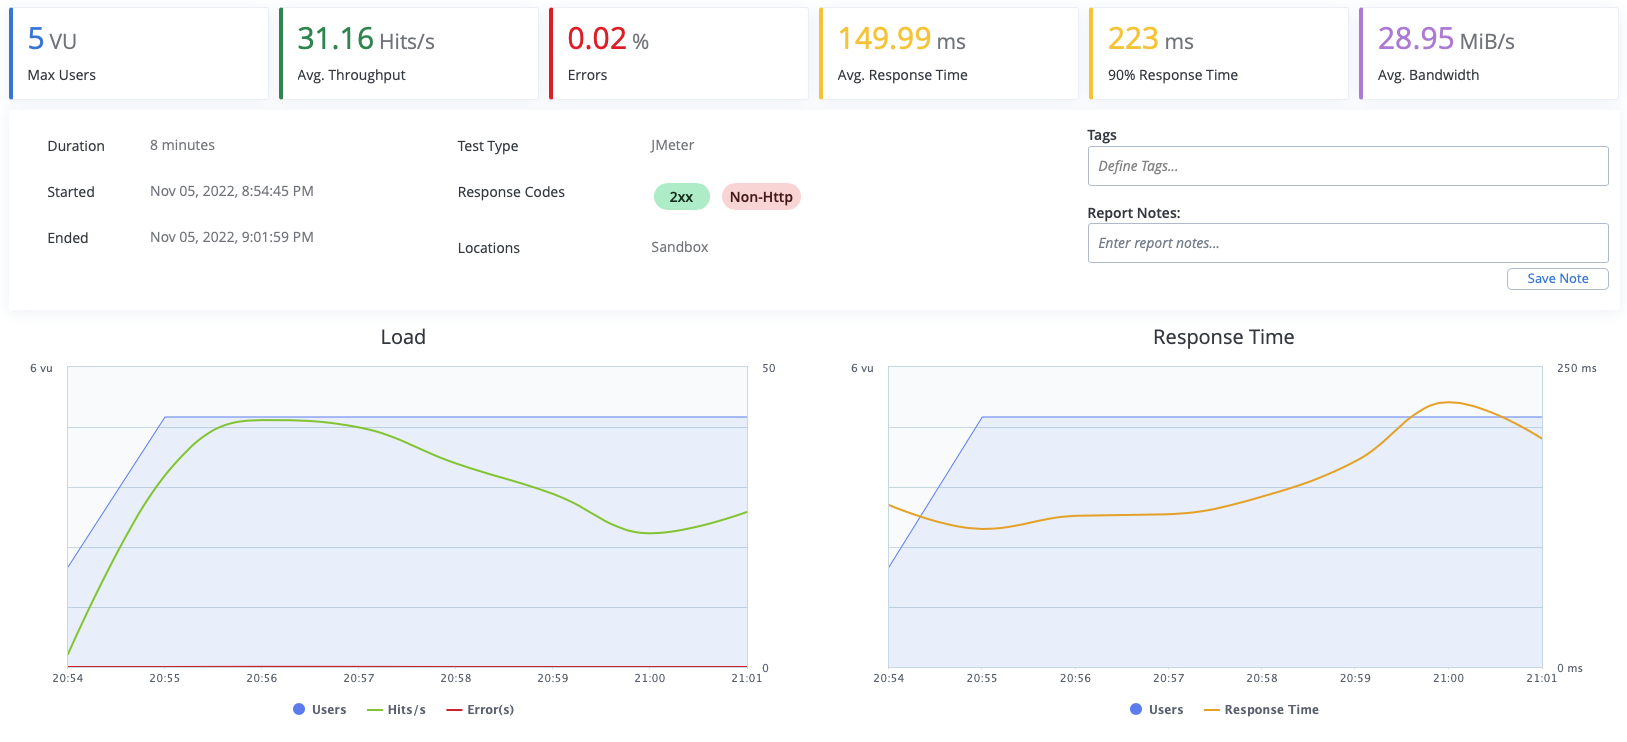
\includegraphics[width=1\textwidth]{gfx/prueba1.png}
    \caption[Prueba de prestaciones con Jmeter]{Prueba de prestaciones con Jmeter.}\label{gfx:prueba1}
\end{figure}

Al analizar el rendimiento nos damos cuenta de varias cosas que ya hemos comentado. Primero, hay que tener en cuenta que los errores son debido a la carga de contenido externo, en este caso imágenes de los artículos de las noticias. Esto se puede arreglar si descargamos las imágenes en vez de cargar el contenido de fuera. En general el rendimiento de la página es aceptable para la carga proporcionada, aunque el rendimiento puede llegar a ser cuestionable debido a la cantidad de JavaScript proporcionado por la visualización de las gráficas.

\vspace{0.3cm}

Podemos ver también otros benchmarks que analicen nuestra página web. En este caso he elegido \textit{PageSpeed Insights}. En este benchmark, se puede comprobar cómo se han respetado las buenas prácticas, la accesibilidad y el SEO (parámetros de buscadores). Aunque podemos ver que el rendimiento decae debido a los problemas comentados anteriormente (latencia y JavaScript).

\begin{figure}[H]
    \centering
    \myfloatalign
    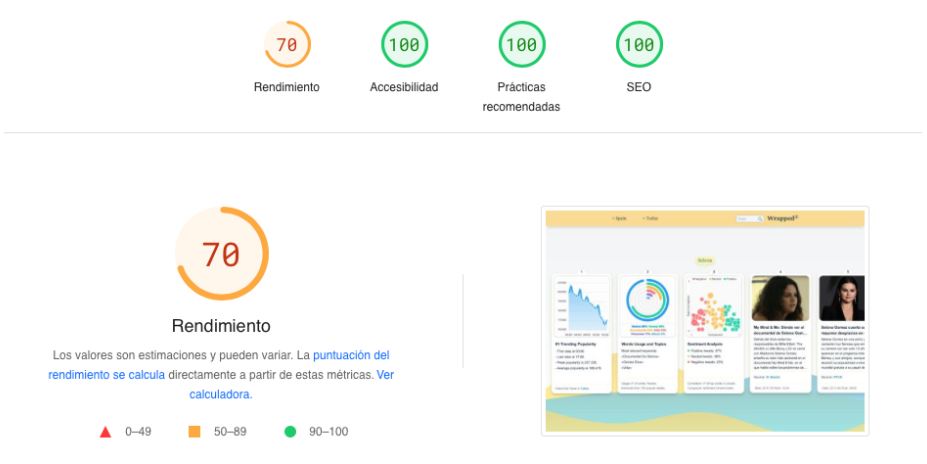
\includegraphics[width=1\textwidth]{gfx/prueba0.png}
    \caption[Prueba de prestaciones con \textit{PageSpeed Insights}]{Prueba de prestaciones con \textit{PageSpeed Insights}.}\label{gfx:prueba50}
\end{figure}

\section{Trabajos futuros}
Como mejora del producto, creo que se puede seguir perfeccionando el contenido de la propia aplicación. Un ejemplo de ello puede ser añadiendo más países o diversificando el contenido, añadiendo vídeos como otro medio de visualización de la tendencia. Los vídeos pueden pertenecer tanto a la propia plataforma de Twitter o a plataformas como YouTube o Vimeo. 

\vspace{0.3cm}

Otra mejora a tener en cuenta es la monetización, esta se puede llegar a integrar como un módulo o carta dentro de la propia aplicación (algo que tenga relación con la tendencia) o directamente cobrar por cada redirección a la noticia u otro enlace que pueda ser monetizado.

\vspace{0.3cm}

Aunque, a mi parecer, las mejoras más importantes a tener en cuenta son las que están relacionadas con la elaboración del proyecto. Se puede seguir mejorando la arquitectura de la aplicación, hacer que sea más escalable y buscar otras vías que no sean las plataformas de servicio \ac{PaaS} gratuitas, de esta manera se mejoraría notablemente la latencia.

\vspace{0.3cm}

Otra cuestión de importancia, es mejorar el rendimiento en la interfaz de usuario. En la sección anterior se ha comentado la posibilidad de cambiar de \textit{framework}, se podrían hacer pruebas de rendimiento o prestaciones con distintos \textit{frameworks} que tengan el DOM estático (como Svelte) o virtual (como Vue o React), de esta manera comprobar cuál es más eficiente con mi aplicación. Aunque se hayan hecho estudios técnicos sobre distintos \textit{frameworks}, no es lo mismo que ver cómo se comporta mi aplicación en cada uno de ellos.

\vspace{0.3cm}

Incluso se podría comparar el rendimiento con otra librería de gráficos y áreas. También se ha comentado la posibilidad de incorporar vistas de esqueletos a la aplicación, aligerando así la carga de contenido cambiante. Incluso se podría incorporar algún tipo de paginación, de manera que solo se cargue el contenido que vea el usuario.

\vspace{0.3cm}

Como última aportación creo que es importante perfeccionar primero o anteponer las posibles mejoras comentadas sobre la estructura de la aplicación, que seguir agregando contenido nuevo o formas de monetización. De esta manera conseguiríamos una aplicación mucho más robusta y escalable, la cual no nos daría problemas en el futuro a la hora de agregar implementaciones nuevas.